%-------------------------------------------------------------------------------
% Introduction to the chapter
%-------------------------------------------------------------------------------

\section{Medium Data Toolkit}

\textsc{Big data and its analytics} promises huge benefits in terms of value realisation, cost reduction, insights but it also introduces a numerous pitfalls \cite{gandomi2015beyond}.
With developments in information technology, mobile communications and internet of things, large assemblages of data are readily available leading to immense possibilities in research.
But when we analyse these data at such scale, we also encounter a large amount of added complexity and cost.
Hence it is important to be careful in choosing the methods and tools in dealing with big data where we should look to devise right methods and tools for the right problems.
Moreover in several disciplines, such as statistics and geography etc., the existing methods and tools are already developed for dealing with large scale data.
These methods along with improvements in hardware has made the processing big data in these disciplines possible without a major changes in workflow.
In the current environment of constant change and growth of sources of data, we cannot afford to lose the opportunity to extract information from them while trying to create a perfect, future proof approach in dealing with them.
We need to move fast with a pragmatic approach where we look at other disciplines and adopt best practices and solutions in them and develop consistent approach for our needs rather than reinventing the wheel.

%-------------------------------------------------------------------------------

In the previous chapters we looked at various methods we devised to collect and process data from Wi-Fi probe requests emitted by phones.
Though we discussed the methods conceptually, we left out the rationale behind choosing the toolkit employed to implement those methods.
In this section we elaborate the thought process and rationale behind these decisions.
We start by discussing the concept of `Big Data' in general and look at previous literature to understand its definition, nature and the challenges they pose.
Then we look at the data-sets we collected through the pilot studies and the `Smart Street Sensor' project and evaluate them in terms of the dimensions of the big data.
We also discuss the challenges faced in dealing with our dataset in detail and try to understand the requirements for devising a toolkit for it.
Finally we put together a toolkit to suit our datasets built from simple small UNIX tools. \sidenote[][-1cm]{"Write programs that do one thing and do it well. Write programs to work together. Write programs to handle text streams, because that is a universal interface.", Doug McIlroy on UNIX philosophy.}

%-------------------------------------------------------------------------------
% Discussion on what is big data
%-------------------------------------------------------------------------------

\subsection{What is `Big Data'?}

With the proliferation of internet enabled personal devices, we have quickly moved from data sparse environment to a data rich one.
We can even confidently say that we are in an age of data deluge where the amount of data which are collected and stored are increasing exponentially in a very short period of time \cite{kitchin2014big}.
As we saw in the previous chapters collecting large amount of data is quick and easy.
Technological advancements have enabled us to be able to think about utilising such large assemblages of data which would have been impossible even in the recent past.
By providing unprecedented coverage, these large assemblages of data - `Big data', provide us with insights which were not possible before.
They often change our approach and methods employed in entire disciplines.
For example, In computer science, fuelled by the explosion of collected user data, there is a paradigm shift in Artificial Intelligence with the use of data mining, machine learning and deep learning.
It is only time before this approach pervades social sciences research as well.
In addition to the above advantages, Big data because of their nature also introduce numerous challenges in their collection, storage, analysis and visualisation.
This is not including the enormous additional overhead and complexity introduced when we try to employ big data methods and tools.
If we are not careful, using big data tools and methods for solving 'normal' problem can be counter productive where the advantages realised don't justified the overheads introduced.
Hence it is important to understand the `Big data' nature of the datasets we are dealing with at a granular level and choose the tools and methods without any presumptions.

%-------------------------------------------------------------------------------

The first and foremost challenge we face while discussing big data is its definition.
It is hard to clearly and objectively define `Big data' as it can vary widely based on the discipline and perspective.
What may be `big' in one discipline may not be in another.
The nature of data can also be evaluated in various dimensions and can exhibit different properties in those dimensions. 
`Big data' is generally defined within the context of disciplines, as data which cannot be managed with traditional methods and tools in those disciplines and requires substantial change in the approach of the practitioners.
This definition is too subjective and falls short of giving us more understanding of `Big data'.
One of the most subscribed definition is to define the scale of the data in the dimension of volume - size of the data, velocity - speed of the data and variety  - the complexity of the data \cite{laney20013d}.
This has also been extended to include more dimensions such as, veracity - the reliability or truthfulness of the data, visualisation - the complexity in visual interpretation and presentation of the data, and others such as visibility validity, variability, volatility and value.
There have also been other alternative dimensions proposed such as Cardinality, continuity and complexity \cite{suthaharan2014big}.
However we can consider the core dimensions of data - volume, velocity, variety, veracity and visualisation for evaluating our datasets.
Since not all data is 'Big' in all these dimensions, we need to evaluate the `bigness' of the data in each dimension and consider the associated challenges and solutions.

%-------------------------------------------------------------------------------

The second set of challenges arise while we process the big data, its acquisition, storage, extraction, cleaning, annotation, integration, aggregation, modelling, analysis, visualisation and interpretation.
Challenges in each one of these processing activity arises due to the data being big in one or more dimensions.
The data being big in volume, velocity and variety poses challenges in data acquisition, aggregation, cleaning and analysis \cite{li2016geospatial}. 
These challenges make traditional methods impractical and introduce the need for distributed, crowdsourced collection of data, heavily parallelised computing and application of functional programming concepts.
The unstructured nature of the big data also introduces notable biases which mandate careful consideration, proper calibration and weighting during analysis so that we can understand and remove any uncertainties arising from them.
The data being big in veracity dimension poses significant challenges in its analysis and modelling.
Since simple methods such as linear regression fails in such scenarios, we require complex methods such as support vector machines, neural networks and hidden Markov models which compensate the lack of structure with the volume of data.
With such computationally intensive methods, heavily parallelised high performance computing techniques such as GPU processing become indispensable.
We also face significant challenge in visualising such complex features and methods which not only supports critical decision making but also is indispensable in exploratory analysis.
The volume and velocity of big data makes them hard to visually simplify and digest.
They are especially complex to interpret in the time dimension unless presented in small parts.
Geographic information systems do a good job in visualising complex geographic data but struggle to maintain legibility and meaning when dealing with the temporal dimension.
The visualisations of big data need to be highly processed, simplified and interactive to present meaning to the viewer. 
They have to balance between functionality, aesthetics and performance.
Finally, because of the variety, big data creates need for consistent, well engineered standards so that multiple approaches and tools can be employed in tandem.

%-------------------------------------------------------------------------------

Apart from these processing challenges, we also have management challenges associated with big data such as privacy and security, data governance and ownership, data and information sharing, and cost\cite{jagadish2014big}.
Since these big datasets are usually comprehensive, securing them and protecting the privacy of the users becomes a central consideration in any project dealing with them.
In many cases, though the data collected itself may not contain personal information but at these scales, in conjunction with other datasets, it can be used to infer them.
The overall approach, methods, tools should comply with relevant legislation such as GDPR as well as the research ethics of all the stakeholders.
This is especially challenging since these large unstructured datasets exhibit ambiguity of their ownership as well which calls for a clear, transparent and secure way to share them with other stakeholders along with publications of results in a timely, accessible manner.
The associated project management and tracking tools need to be capable of handling these data ownership and sharing concerns as well.

Finally, the biggest challenge we face with big data is the cost in terms of money, resources and time.
Though most of the big data tools are developed openly and distributed freely there can be lot of incidental, non-direct costs associated with collecting, processing and managing data with them.
For example, there are the operational costs collecting data at such scale, network costs moving them, server costs storing and processing them, cost of procuring and supporting specialised tools and the human resource cost in hiring and training people who are capable for dealing with them.
Though there are economies of scale at larger scales, the overall resources required to manage big data effectively can be several folds of what is needed for a traditional dataset. 
This makes it important to look at the data in our hands closely and carefully so that we can make informed decisions on how 'big' it is and choose the methods which are the most suited for such dataset.

%-------------------------------------------------------------------------------
% Discuss the data we have in detail 
%-------------------------------------------------------------------------------

\subsection{How big are the Wi-Fi probe request datasets?}

In this section we take a detailed look at the three sets of Wi-Fi probe requests collected as described in chapter on data collection using the 5Vs big data framework.
Our aim is to understand the nature of the data in each dimension and thus evaluate the challenges we face in that specific dimension leading to a bespoke solution.
We look at each set of data in each dimension and try to answer the following questions,

\begin{enumerate}
  \setlength{\itemindent}{2em}
  \itemsep-0.25em
  \item{How can this dimension be measure objectively?}
  \item{How big is the data in terms of the defined measurement?}
  \item{How does it data compare with datasets in other disciplines?}
  \item{How can we describe the size of the data?}
\end{enumerate}

We then combine these isolated evaluations to form a combined description of the datasets. This is then used as the basis for developing a list of requirements for designing the data processing and management toolkit.

%-------------------------------------------------------------------------------

\vspace{1.5em}\noindent\textit{Volume}\vspace{0.5em}

\noindent Probe requests data, being dynamic and continuous, cannot be quantified as an absolute static number in terms of volume. 
Hence we use a long term measurement - yearly rate, for each location instead.
On shorter datasets such as the pilot study, we estimate the yearly volume linearly from the available data.
We standardise this measure as the amount of disk space needed to store the collected data when encoded in text form.
It is important to note that this can be reduced many folds by using compression or binary formats but we chose text since it the de-facto standard for exchanging data.

\begin{table}[h]
  \footnotesize
  \begin{center}
    \begin{tabular}{lcccc}
      \toprule
      Study & Maximum* & Minimum* & Average* & Total** \\
      \midrule
      Pilot Study & 134 & 3 & 54 & 48.3 \\
      Main Study & 6.1 & 2.4 & 4.42 & 4.1 \\
      Smart Street Sensor & 5.4 & 0.001 & 0.8 & 0.8 \\
      \bottomrule
    \end{tabular}
  \end{center}
  \caption{Comparison of volume or size of the datasets of Wi-Fi probe requests.}
  \label{table:toolkit:volume}
\end{table}

\marginnote{\textit{* Measured/ Estimated for each location in gigabytes per year. ** Measured/ Estimated for 920 locations in terabytes per year} }

We can see that there is a lot of variability in the volume of probe requests generated at a given location.
This mostly depends on how many mobile devices are present around the location.
We observe that when we collect most of the information present in the probe requests in a busy area such as Oxford street in the Pilot studies, we generate around 50 terabytes of data in a year.
But in a more real world setting such as the Smart Street Sensor project where the sensors fail at times and the amount of data collected is optimised, the volume is around a 1 gigabyte.
The total volume of data we deal with in the case of a national scale project with around 920 sensors running for around 4 years is around 2 terabytes.
A comparison of this to datasets from other disciplines is shown in Figure \ref{figure:toolkit:volume}.
It is key to note that the y-axis is scaled exponentially.

\begin{marginfigure}
  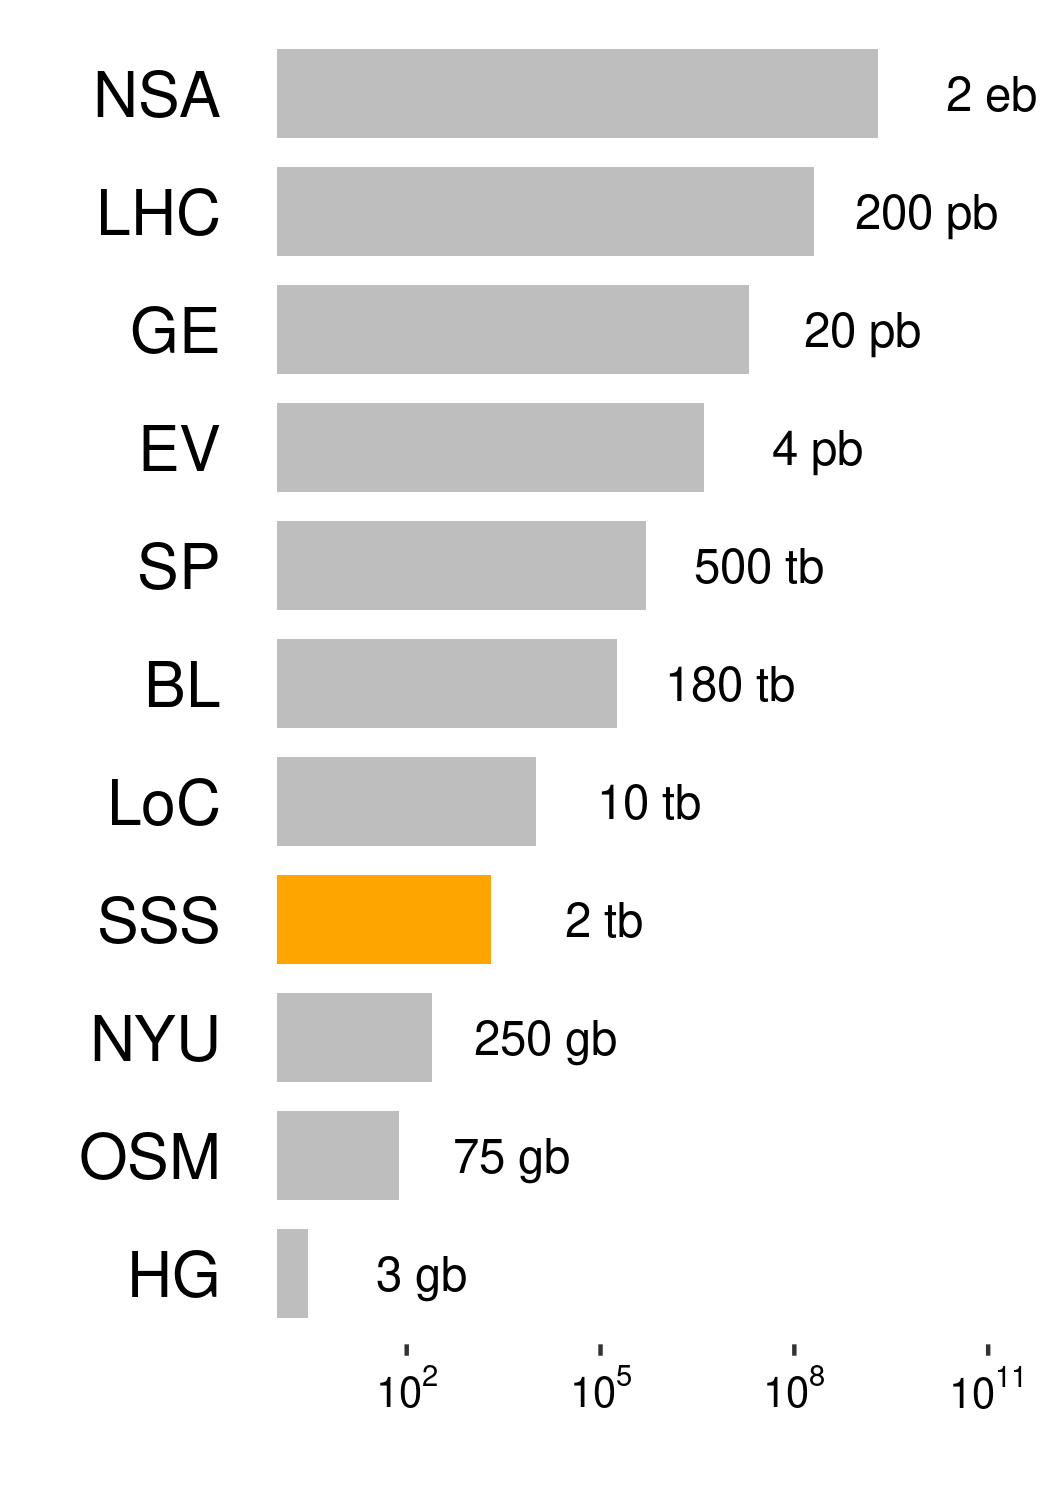
\includegraphics{images/data-size-comparison.png}
  \caption{Comparison of volumes of datasets across various disciplines.}
  \label{figure:toolkit:volume}
\end{marginfigure}

\marginnote[1em]{\fontsize{7}{7}\textit{NSA - National Security Agency, LHC - Large Hadron Collider, GE - Google Earth, EV - Event Horizon project, SP - Spotify music, BL - British Library data store, LoC - Library of Congress, SSS - Smart Street Sensor, NYU - New york city Uber trips 2009-15, OSM - Open Street Map and HG - Human Genome Project}}

We can see that the probe requests data is not truly 'Big data' as experienced in other fields.
It is only when we reach a complete coverage, i.e, putting a sensor at each retail establishment in UK, our estimated data volume reaches around 250 petabytes which is comparable to scales experienced in other fields such as particle physics and world wide social networks.
At the same time, the scale of probe request data is not small either.
The volume of 2 terabytes is more than the memory available in any desktop systems and is more than any of them can process in a timely manner.
Summarising from the above, we can confidently say that the probe request datasets are `Medium Data' - especially the dataset collected by the smart street sensor project.
Though it has potential to scale into a truly big dataset, for the purposes of this research we can classify it as `Medium data' in the volume dimension.

%-------------------------------------------------------------------------------

\vspace{1.5em}\noindent\textit{Velocity}\vspace{0.5em}

Velocity is the rate at which the data is collected over time.
It is significant when evaluating big data since some data which may not scale in terms of absolute volume but the speed at which they are received makes them challenging to deal with.
A perfect example is the comparison between data generated by the Large Hadron Collider project by European Council for Nuclear Research and a world wide social network such as Facebook.
Though their total volumes are comparable at 200 petabytes, the data from LHC is generated in concentrated experiments at a rate of 3 petabytes in 5 seconds while Facebook generates the same about in about a day or two.
Since the size of an individual Wi-Fi probe request doesn't vary widely, we define the velocity of this dataset as the number of requests received at a given location at a given location within a given time interval.
Though the precision of the time measured during data collection is in microseconds, the practical data transfer resolution in all the datasets is around 5 minutes.
Hence we measure velocity of out datasets in terms of number of requests every 5 minutes.
Table \ref{table:toolkit:velocity} compares the datasets we collected on Wi-Fi probe requests in terms of their volume.

\begin{table}[h]
  \footnotesize
  \begin{center}
    \begin{tabular}{lcccc}
      \toprule
      Study & Maximum* & Minimum* & Average* & Total** \\
      \midrule
      Pilot Study & 8577 & 188 & 3469 & 3.20 \\
      Main Study & 1362 & 534 & 782 & 0.72 \\
      Smart Street Sensor & 5024 & 6 & 408 & 0.27 \\
      \bottomrule
    \end{tabular}
  \end{center}
  \caption{Comparison of velocity or speed of the datasets of Wi-Fi probe requests.}
  \label{table:toolkit:velocity}
\end{table}

\marginnote{\textit{* Measured/ Estimated for each location in number of requests per 5 minutes. ** Measured/ Estimated for 920 locations in Millions of requests per 5 minutes} }

We observe that locations can receive up to 8500 requests in 5 minutes or can get no request at all depending on the time and how busy it is.
But we can see that on average a national scale project with around 900 locations generates around a million requests every 15 mins. 
Compared to the LHC's 180 billion records or Google's 190 million searches per 5 minutes this seems to be not high speed data.
However, this is much faster compared to traditional data sources such as census or geographical surveys which are updated anywhere between 6 months to 10 years.

To summarise, in terms of velocity, the Wi-Fi probes data can be described as 'Medium' at best. 
The methods dealing with the data should be time sensitive and be able to deal with a continuous stream of data but at the same time need not be real time or need sub-second latency.
Since the Wi-Fi probe requests don't have actual location information the mobile devices, it does not have the similar value in real-time analytics as shown in comparable location or movement based datasets.

%-------------------------------------------------------------------------------

\vspace{1.5em}\noindent\textit{Variety}\vspace{0.5em}

Variety is defined by the amount of variance in the type and characteristics of the data.
Since variety is hard to quantify and compare across disciplines we evaluate the dataset subjectively for the variety present in it.
The data transmitted in a Wi-Fi probe request is defined by the 802.11 Wi-Fi specification \cite{ieee2016} and every probe request has to have a set of mandatory fields for Wi-Fi to work.
This set of fields is the same everywhere across the world and the specification, especially the probe request part, has remained stable over years.
Though there is some variability allowed within the specification, being part of a global standard, the data collected is heavily structured in general.

The first set of variety present in the Wi-Fi probes data set arises from the 'information elements' part of the probe request.
The structure of a probe request is discussed in detail in the data collection chapter and is summarised in Figure ?.
Essentially the information about the capabilities and type of the mobile device is encoded in the information elements part of the probe request and this information is optional and is implemented at the discretion of the manufacturers.
As this information elements are demonstrated to be useful in successfully fingerprinting the mobile devices \cite{vanhoef2016}, mobile devices increasingly don't include any information in them.
Emergence of manufacturers with large market share and narrow set of device models such as Apple and Samsung also reduce further variability in them.
The second set of variety in the dataset arises from the rate at which these probe requests are generated by the mobile devices. 
Unlike devices which generate data on events or at regular intervals, mobile phones generate probe requests at a rate based on various factors.
Though this leads to some challenges in counting footfall from these probe requests the variability exhibited here is neither so large nor so complex that traditional methods could not deal with them.

Comparing with some of the big data encountered in unstructured data collected over web such as social networks or other sensor based methods, the variability here can be considered trivial.
Further when we convert these probe requests in to footfall counts, the variety in the dataset drops almost to zero as it becomes just an ordinal data point varying in geography and time.
Summarising the above, we can confidently say that the Wi-Fi probe request data does not exhibit any `big data' properties in the variety dimension.

%-------------------------------------------------------------------------------

\vspace{1.5em}\noindent\textit{Veracity}\vspace{0.5em}

Veracity is defined as the amount of abnormality present in the data in the form of inaccuracies, biases and noise.
Similar to variety, veracity is hard to quantify hence required a subjective evaluation.
Being sensor collected data, veracity is the dimension where the data exhibits most `big data' properties.

\begin{marginfigure}
  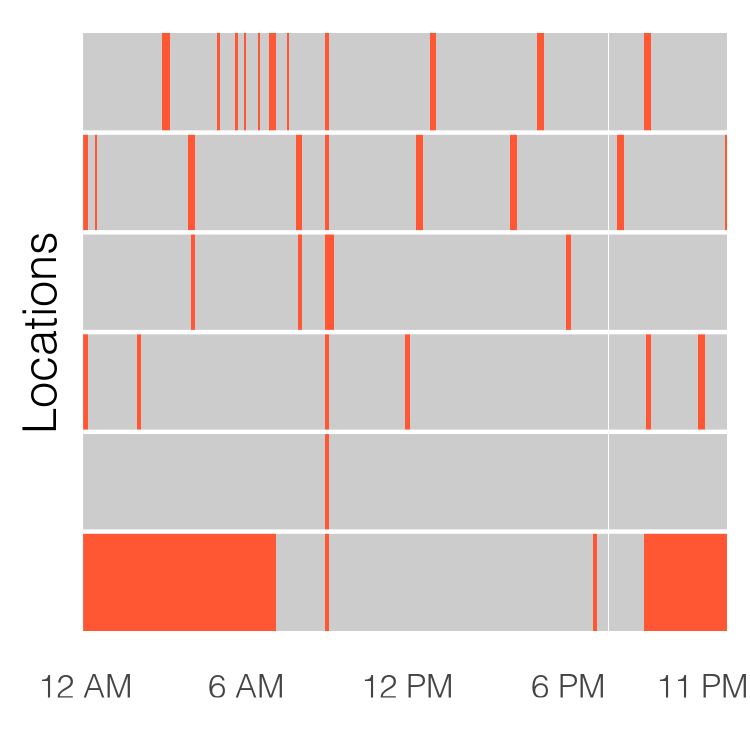
\includegraphics{images/data-veracity-gaps.png}
  \caption{Missing data from five locations at Tottenham Court Road, London on 15 January 2018 demonstrating the veracity of the data.}
  \label{figure:toolkit:veracity:gaps}
\end{marginfigure}

First set of veracity in the dataset arise from the fact that it is collected through sensors located in multiple locations which communicate to the central server using 3G mobile data connectivity.
We know from experience that the sensors are unreliable and fail to send back data regularly due to various reasons.
More over the sensors are installed and uninstalled regularly as partners join and leave the project.
This results in a data stream which is often erratic and incomplete with large gaps in them.
In addition to this the sensors need to be rebooted regularly due to issues or updates leading to small gaps as well.
Since the sensors are part of retail establishments they can be switched on and off regularly in some of them as well.
Figure \ref{figure:toolkit:veracity:gaps} demonstrates the veracity of the data in terms of missing data for a sample of locations in London.
All the above pose immense challenges when we attempt to aggregate the data where we have to estimate and fill these gaps.

There is also a lot of variability in the physical location of the sensors and the area of measurement.
The sensors may report higher or lower count due to their configuration and the context of their location as discussed in chapters pertaining to data cleaning.
This leads to a situation where the accuracy of the data collection varying quite widely across location and times \cite{lugomer2017understanding}.
It is often not clear if the change in the data is due to actual changes at the location or just the change in the configuration of the device.
For example, Opening of a mobile shop next door to the sensor can increase the estimated footfall without any change in actual footfall at the location.

Finally we also have to work within the changing mobile landscape.
Though the Wi-Fi probe requests are standardised by IEEE, the mobile manufacturers have started adopting obfuscation techniques to protect the privacy of the users.
This started with randomisation of MAC addresses, removal of information elements and generally getting more sophisticated with new versions of operating system.
There is also bias in terms of operating system adoption and change in market share between manufacturers.
There is no inherent structure or information on what is changed and how often these changes occur which leads to questions on the continuity of the data over long periods of time.

Summarising from the above, we can confidently conclude that Wi-Fi probe requests dataset shows `Big data' characteristics in terms of its veracity and requires appropriate tools and methods when aggregating, analysing and modelling it.

%-------------------------------------------------------------------------------

\vspace{1.5em}\noindent\textit{Visualisation}\vspace{0.5em}

Visualisation is closely related to volume, velocity and variety of the data.
The Wi-Fi data due to its non-trivial volume and velocity, exhibits similar characteristics and challenges in terms of visualisation.
Since there is not much variety in the dataset, when we process the raw data into footfall counts we are left with just the time, location and footfall count for each data point.
Out of these, location and footfall counts are easy to visualise but time exhibits big data properties.
This is primarily due to its granularity at 5 minute intervals and longitudinal nature of the data collection.
The major challenge with Wi-Fi data is to simplify and visualise them in a legible way while showing change in term of time.
The veracity of the data presents challenges in simplifying them and the volume poses challenges in maintaining legibility.
We also have to take the `near real time' aspect of the data into consideration while visualising them.
There is a clear need for always on, interactive, real time dashboards with geographic capabilities in addition to the capabilities of traditional desktop GIS.
There is also need for multiple linked dynamic visualisation platform for separating the scope of the visualisation into manageable units.
Figure \ref{figure:toolkit:visualisation} demonstrates the illegibility of simple visualisations of the data due to granularity, variability and veracity.
We can safely say that the Wi-Fi probe requests dataset is at best `Medium' in the visualisation dimension.

\begin{figure*}
  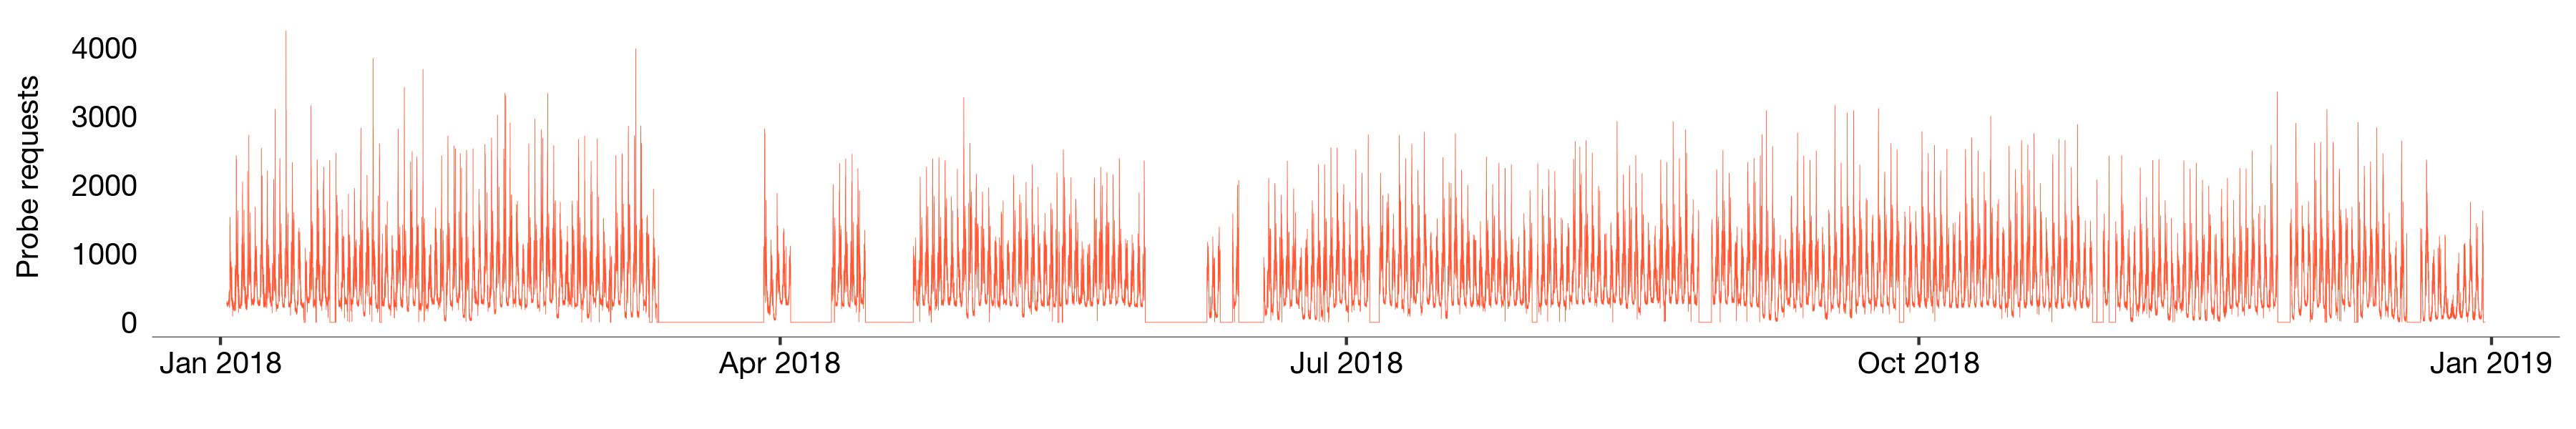
\includegraphics{images/data-visualisation-challenge.png}
  \caption{Number of probe requests collected for every five minute interval at Tottenham Court Road, London on the year 2018.}
  \label{figure:toolkit:visualisation}
\end{figure*}

Summarising the above discussion, we can conclude that the datasets collected from Wi-Fi probe requests are at best of 'medium'.
They show the most big data characteristics in terms of their veracity.
In rest of the dimensions the datasets are not truly big data and we need to look at tools and methods appropriate to their size.
The toolkit we devise need to be able to deal with their mid-size volume, velocity and visualisation dimensions and at the same time need to able to deal with the large amount of veracity of in them.
Figure \ref{figure:toolkit:spider} illustrates the summary our discussion.
This leads us to devise a `medium data toolkit' which can be used without incurring the extra cost and complexity introduced by big data tools while be able to handle the data at hand.

\begin{marginfigure}[5cm]
  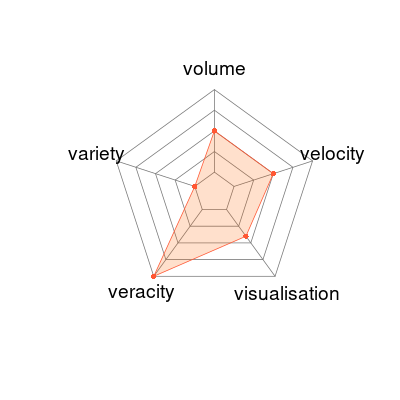
\includegraphics[trim={2.1cm 0 0 0},clip]{images/spider.png}
  \caption{Big data characteristics of the Wi-Fi probe request datasets in their corresponding dimensions}
  \label{figure:toolkit:spider}
\end{marginfigure}

%-------------------------------------------------------------------------------
% A survey of all tools and methods dealing with big data.
%-------------------------------------------------------------------------------

\subsection{A Survey of Methods and Tools}

Having classified the Wi-Fi probes dataset as a `Medium' sized data, in this section, we survey the tools and methods available at various stages of the data processing and management process - data collection, storage and retrieval, processing and analysis, visualisation.
We first survey the tools available in each stage and specifically look at their suitability for Wi-Fi probe request datasets in terms of the following characteristics,

\begin{itemize}
  \setlength{\itemindent}{1em}
  \itemsep-0.25em
  \item \textit{Performance} - How much data can be processed in a given time?
  \item \textit{Flexibility} - How easy it is to change the scale and scope?
  \item \textit{Complexity} - How many components/parts are involved?
  \item \textit{Cost} - How much money/ infrastructure do they require?
\end{itemize}

We then discuss the principles of UNIX philosophy and how it helps in solving similar sized problems in computer science. Finally we pick and connect the tools to devise our toolkit which is best suited for out Wi-Fi probe request dataset.

%-------------------------------------------------------------------------------

\vspace{1.5em}\noindent\textit{Collection}\vspace{0.5em}

There are numerous tools available for data collection with network of sensors under the umbrella of internet of things.
The primary consideration in the data collection is the scale of the infrastructure and the cost associated with it.
The smartstreetsensor project uses its own proprietary sensor system which collects data at the location.
The tooling decisions were made with the commercial application in mind and is not entirely relevant to our discussion, but for the research conducted with the data, it is necessary to understand the data collection process and how the toolkit integrates with the rest of the setup.
We start by looking at different approaches in the data collection tools and try to reason the most appropriate solution for the Wi-Fi data.
At the hardware level, the lowest level of tool can be a micro-controller such as audrino with a dedicated hardware module with custom software to collect the exact data needed.
This is time consuming, cumbersome takes a lot of cost to develop, but is very flexible, efficient and cheap to deploy.
On the other end of this spectrum we have end-to-end solutions such as Blix, Walkbase, Ecuclid, Retail next, pygmalios etc where the data set is collected through multiple sources and syndicated into a cleaned source by a thirdparty.
This can be costly and inflexible but quick and easy.
The middle ground on this to deal with a complexity as much as the Wi-Fi data, is to use a single board computer with external modules and use general purpose, tools to build a data collection device.

The toolkit we have adopted consists of RaspberryPi, Linux, tcpdump/tshark and nodejs.
The RaspberryPi and the linux platform it provides is one of the most diverse and general purpose systems available.
On top of which we can build our data collection system with specialised, opensource and free Wi-Fi sniffing tool such as tcpdump, tshark along with a general purpose runtime such as nodejs which provides other functions such as scheduling, personal data obfuscation and data transmission.
This system has a capacity to sniff and transfer large amounts of data and with a 3G module is very versatile in terms of location.

%-------------------------------------------------------------------------------

\vspace{1.5em}\noindent\textit{Storage}\vspace{0.5em}

This is one of the most diverse set of area in terms of both methods and tools available.
It has been constantly in development since the beginning of computer systems and is one of the fastest changing landscapes.
The aspects to be considered while choosing the data storage solutions are,

\begin{enumerate}
    \item Speed
    \item Redundancy
    \item Reliability
    \item Cost \& complexity
\end{enumerate}

One of the spectrum is just using file systems for storage.
Though it seems to be primitive, this has a lot of advantages.
Operating systems usually are really good at managing - reading, writing and searching filesystems, They usually have no overhead involved and are efficient.
Hierarchical organisations can be pre-indexed for hierarchical data and finally is very reliable.
But the primary disadvantage is the inability to handle complexity or variety in data.

On the other end of the spectrum is the highly distributed big data systems such as Hadoop HDFS which are built for > petabyte datasets and query them without loss of speed.
There are hybrid file systems which are hadoop compatible as well, Azure blob storage, Amazon S3 cloud storage which can be used a storage/ dump for a large amount of data.

In the middle there are databases, which are built prioritise and balance the database needs.
The two major approaches are the relational databases which are optimised for structured data which are related to each other in tabular format.
They are row heavy databases and are good for high volume, low veracity data which has need for consistency.
SQL databases PostgreSQL, Mysql, SQLserver are examples.
The other approach is the document store databases which are column heavy databases which are optimised for high variety data which doesnot need immediate consistency.
These can be as simple as key-value based databases and as complicated as graph databases.
Mongodb, couchdb, cassandra as examples.
Both these approaches can be scaled/distributed for less redundancy and increased throughput.
The former tend to scale veritcally and the latter scale horizontally.
Some like cassandra are built to be highly distributable.

Finally there are solutions such as Hive and hbase which are database like functionality built on top of distributed file systems combining power of both concepts.
This behaves like a hyper large scale database system and works in conjunction with other big data tools


\begin{table}[h]
  \footnotesize
  \begin{center}
    \begin{tabular}{ll}
      \toprule
        Type & Comment\\
      \midrule
        Filesystem & for hierarchical data around 10TB range\\
        Cloud Storage & \textless{}  10TB, can add hdfs stuff, more reliability\\
        Relational DB & 1-5TB, Good for relational Data, Row-wise, Partitioning\\
        Document DB & -10TB, Good for unstructured data, column wise,Clustering\\
        HDFS & \textgreater{} 10 TB, Good for scale and structure\\
        Hive, Hbase & on top of HDFS, bring DB to HDFS\\
      \bottomrule
    \end{tabular}
  \end{center}
  \caption{Types and Use of Various Storage Solutions}
  \label{table:toolkit:storage}
\end{table}


Raw wifi data has temporal hierarchy and is of medium size hence a normal filesystem is sufficiently suitable for its needs.
When the same data is aggregated it loses its scale and is highly strucutred so a relation DBMS is sufficient for it.
In case the project runs longer and more longitudinal analysis had to be done on raw data HDFS needs to be used and if the aggregated data scales to >10TB we can handle it with a timescale db should be suitable.
PostgreSQL is more suitable than other databases because of its better support to geographic data.

%-------------------------------------------------------------------------------

\vspace{1.5em}\noindent\textit{Processing}\vspace{0.5em}

The primary considerations while surveying are the volume, velocity and veracity
of the data.
We should be careful to choose the tools which are right for the size.
The perfect tools for a medium size data can be as much as 230x faster than big data tools (ref).
At one end there are Big Data analysis tools such as Hadoop based impementations such as Mapreduce and Spark, Business toosl such as skytree, realtime tools such as storm and samoa, cleaning tools such as Openrefine.
All these tools are optimised for the cluster/grid computing and the processing is heavily parallelised across the clusters.
There is also a lot of overhead asssociated with moving data across clusters and we won't be making up for these overheads until we hit certain size of the data.
As we know Wi-Fi data is not at the scale these tools operate, we can look into how large streams of data are handles in computer science/ systems engineering.
Data processing is done in two stages, the first one is the filtering, cleaning and aggregation of the raw Wi-Fi data and the second step is the analysis and modelling of the aggregated data.
As we saw in (ref) the system tools in combination with parallel processing across CPU cores, can be used and can be actually faster for medium sized data.
The data transfer format is text since it is standardised with utf8 and is easily understood and shared between UNIX tools.
This also helps us in the data sharing and management which is discussed later.
For the first part of the processing - filtering \& cleaning we use the following tools,

\begin{enumerate}

  \item \textbf{sed} - streaming text editor. A fully featured text editor which works on  stream of text. The stream is processed usually by each line and is the most  commonly used to search and replace (translating) text streams using regular  expressions.

  \item \textbf{grep} - grep (global regex print) is a special case of sed where we search  the stream for regular expression and print the result. This is usually used  for searching and filtering text streams.

  \item \textbf{awk} - This is a turing complete special purpose higher level programming  language which is optimised for sorting, validating and transforming text  streams. It is full featured enough to be able to manage a small text based  database by itself. This is usually used to transform tabular delimited data.

  \item \textbf{jq} - This is similar to awk, has a emcascript based scripting language  for transforming text data which is in the JavaScript Object Notation format. These four tools form a core toolkit for tranforming, translating and  filtering data. All these tools are single threaded and need an external tool  to parallelise the processes. For this we can use gnu-parallel.

  \item \textbf{parallel} - This is a tool built with perl (citation) which parallelises  the any operation across CPU cores and even across multiple nodes through  secure shell (ssh). This gives us a medium sized cluster which is well suited  dealing with text data stored in a file system.

\end{enumerate}

Bash completes the toolkit to provide a overarching high-level scripting interface to combine all the smaller tools and managing data transfer between them as text streams using the 'pipe' operator.
This along with core bash tools such as sort, uniq can give us a basic data filtering, transformation and aggregation toolkit with a reasonable throughput.
Example, For a normal word count problem, this toolkit can give us a through put of 540MB per minute without parallelisation and with parallelisation this can be improved to 2.5GB per minute.


For complex data cleaning techniques such as filling in the gaps, we can use higher level languages such as R or Python through their scripting environments and linking them to our pipelines using bash.
Security in terms of obfuscation can be done through hashing algorithms implemented by openssl, nodejs and R and for encryption, we can use the gnupg.
The toolkit being open source free software has the added advantage of being secure as well.

%-------------------------------------------------------------------------------

\vspace{1.5em}\noindent\textit{Visualisation}\vspace{0.5em}

Tableu, Omniscope.

%-------------------------------------------------------------------------------
% Discussion and conclusions
%-------------------------------------------------------------------------------

\subsection{Conclusions}

To summarise we have done a survey of tools and arrived at the following toolkit

Figure of the data toolkit.
